\documentclass[12pt,a4paper]{article}

\usepackage[utf8]{inputenc}
\usepackage[T1]{fontenc}
\usepackage{lmodern}
\usepackage{amsmath,amssymb}
\usepackage{geometry}
\usepackage{graphicx}
\usepackage{xcolor}
\usepackage{booktabs}
\usepackage{array}
\usepackage{hyperref}
\usepackage{float}

\geometry{margin=0.8in}
\setlength{\parskip}{0.6em}
\setlength{\parindent}{0pt}

\definecolor{navy}{HTML}{0F172A}
\definecolor{sky}{HTML}{0284C7}
\definecolor{skybg}{HTML}{E0F2FE}
\definecolor{emerald}{HTML}{15803D}
\definecolor{emeraldbg}{HTML}{DCFCE7}
\definecolor{crimson}{HTML}{B91C1C}
\definecolor{crimsonbg}{HTML}{FEE2E2}
\definecolor{amber}{HTML}{B45309}
\definecolor{amberbg}{HTML}{FEF3C7}
\definecolor{slatebg}{HTML}{F8FAFC}
\definecolor{slateborder}{HTML}{CBD5E1}

\hypersetup{
  colorlinks=true,
  linkcolor=sky,
  urlcolor=sky
}

\newcommand{\calloutbox}[4]{%
  \vspace{0.3em}
  \noindent\fcolorbox{#1}{#2}{%
    \parbox{\dimexpr\textwidth-2\fboxsep-2\fboxrule\relax}{%
      \vspace{0.25em}
      {\large\textbf{\textcolor{#1}{#3}}}\\[0.35em]
      #4
      \vspace{0.25em}
    }%
  }
  \vspace{0.3em}
}

\title{\vspace{-1.2em}\textbf{\LARGE How Nature Builds 10,000 Different Fishes}\\[0.4em]
\Large The Visual Guide for Everyone (13-Year-Old Level with Diagrams)\\[0.3em]
\normalsize Why a 109-Year-Old ``Rubber Graph-Paper'' Idea Was Right --- And Why Computers Missed It}

\author{\textbf{Infinite Morphospace Project} $\cdot$ \texttt{https://github.com/fractastical/morpholib}}
\date{October 22, 2026}

\begin{document}
\maketitle

\calloutbox{navy}{amberbg}{The 60-Second Story in One Sentence}{%
\textbf{Global growth rules (D'Arcy Thompson's curved rubber sheet) shape the \emph{outside} of the fish for swimming over 150 million years, while competition with neighbors rewires the \emph{jaws and snout} on the inside ($3\times$ to $9\times$ faster) so sister species can share the same coral reef without fighting over the same food.}
}

% ============================================================================
\section*{Step 1: D'Arcy Thompson's 1917 ``Rubber Graph-Paper'' Idea}

In 1917, a Scottish scientist named \textbf{D'Arcy Thompson} asked a simple question: \emph{When one fish species evolves into another, does nature have to redesign every single bone from scratch?}

He drew a parrotfish (\emph{Scarus}) on flat graph paper, bent the grid lines into curved circles like a \textbf{sheet of rubber}, and showed that the drawing turned into an angelfish (\emph{Pomacanthus}). He argued that an embryo only needs to turn a few global \textbf{``growth knobs''} (stretching, slanting, or curving the whole body at once) to transform one body plan into another.

\begin{figure}[H]
  \centering
  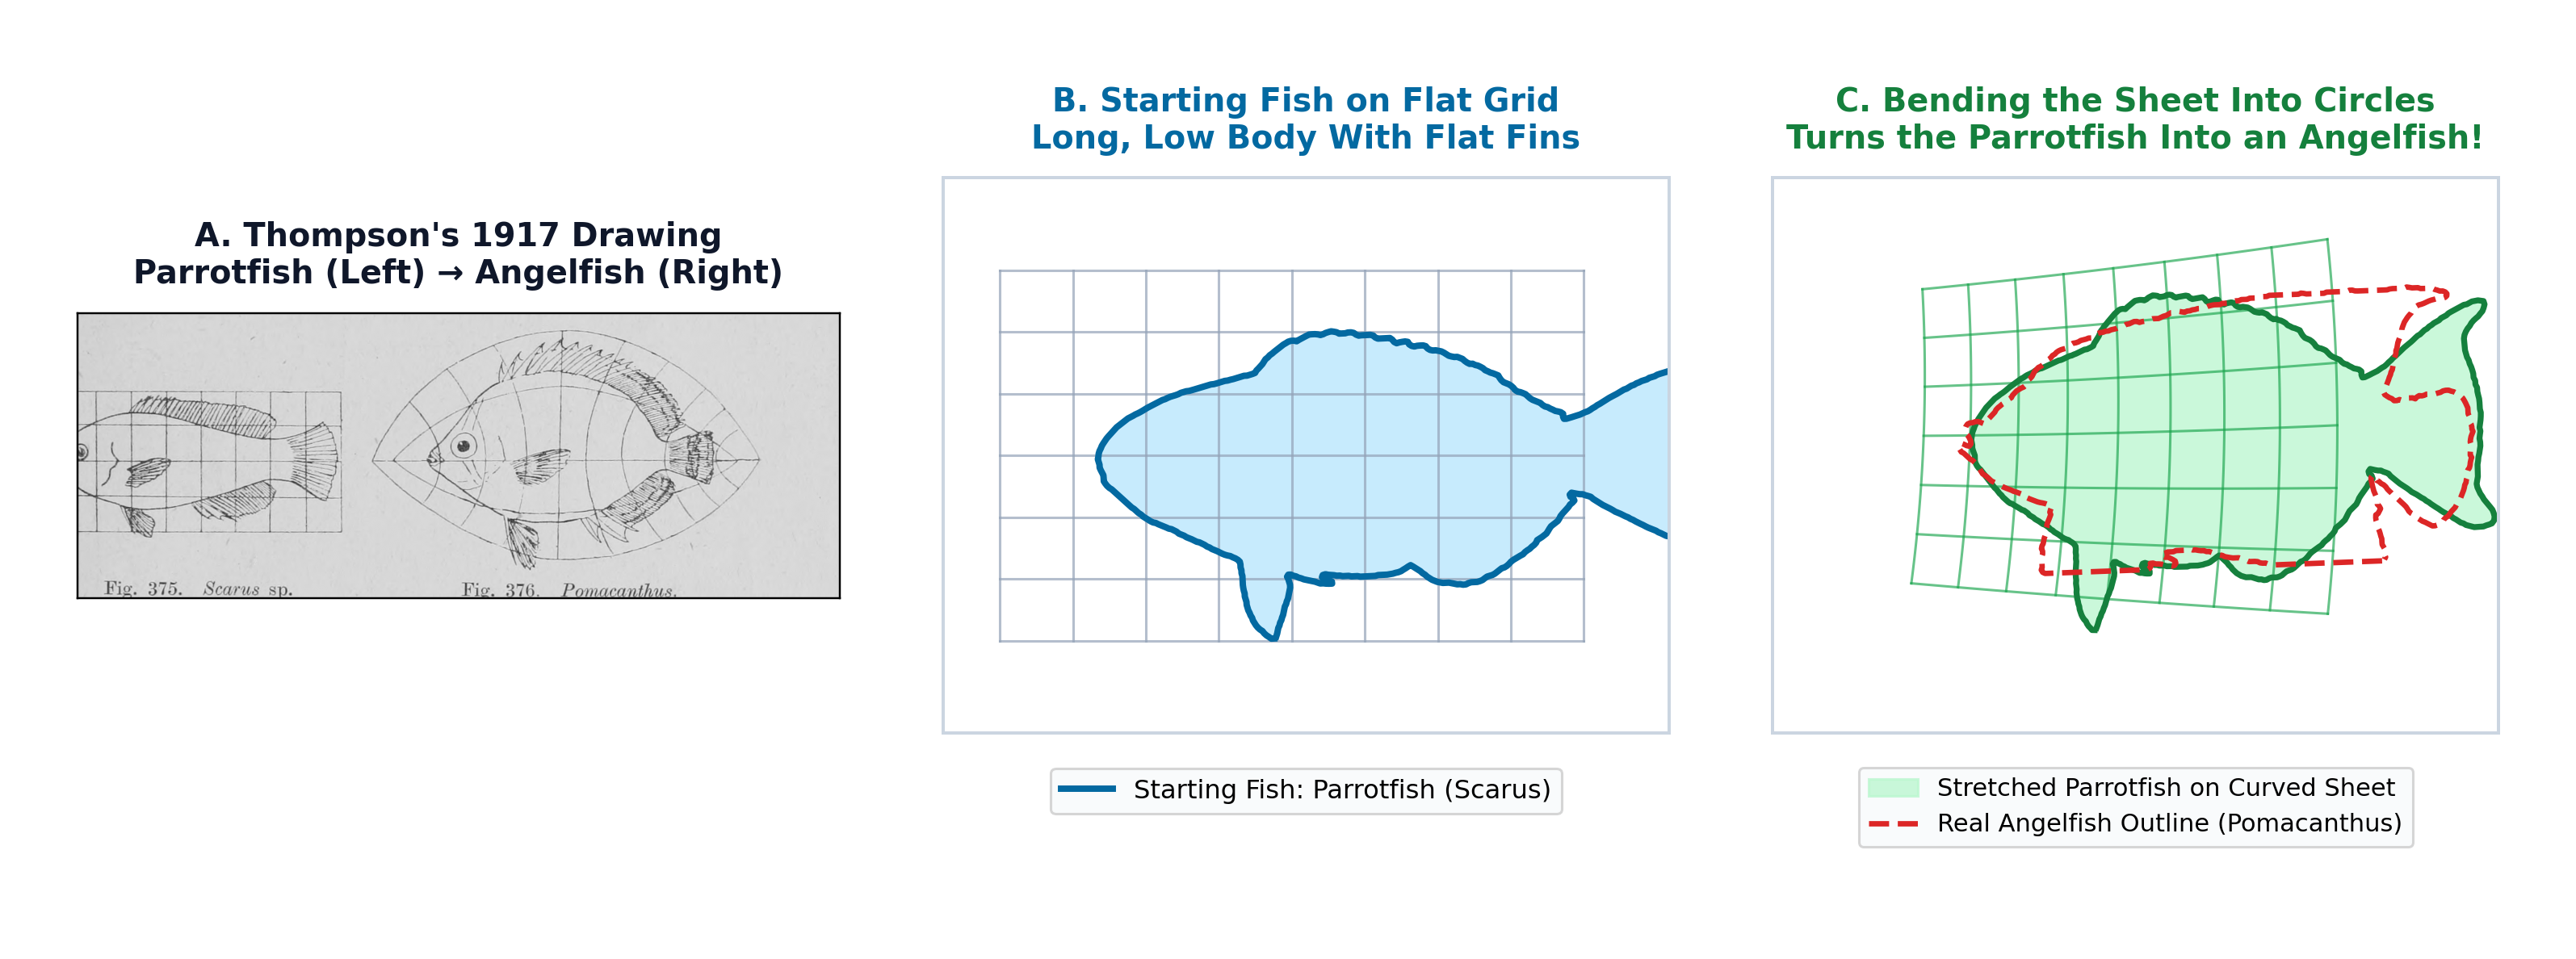
\includegraphics[width=0.99\textwidth]{guide_step1_1917_rubber_sheet.png}
  \caption{\textbf{Step 1 --- D'Arcy Thompson's 1917 Rubber Graph-Paper Idea.} \textbf{(A)} Thompson's original 1917 drawing (p.\ 749). \textbf{(B)} A parrotfish on flat graph paper. \textbf{(C)} Bending the graph paper into coaxial circles transforms the parrotfish silhouette into an angelfish.}
\end{figure}

\newpage
% ============================================================================
\section*{Step 2: Mistake \#1 --- Why Computers Thought Thompson Was Wrong (``The 17-Dot Head Trap'')}

For the last 30 years, biologists tested Thompson's idea on computers and concluded it didn't work across different fish families. \textbf{Why did their computer tests fail?}

Because instead of tracing the \textbf{whole outline of the fish}, standard fish databases only measure \textbf{17 dots on the skeleton}:
\begin{itemize}
  \item \textbf{9 of those 17 dots ($53\%$ of the math weight) are crammed inside the head and jaws} (the yellow circles in Panel A below).
  \item The other \textbf{8 dots ($47\%$)} only mark where the bases of the fins touch the body wall (green squares).
  \item \textbf{Zero dots ($0\%$) are on the actual outer fins or tail!}
\end{itemize}

\begin{figure}[H]
  \centering
  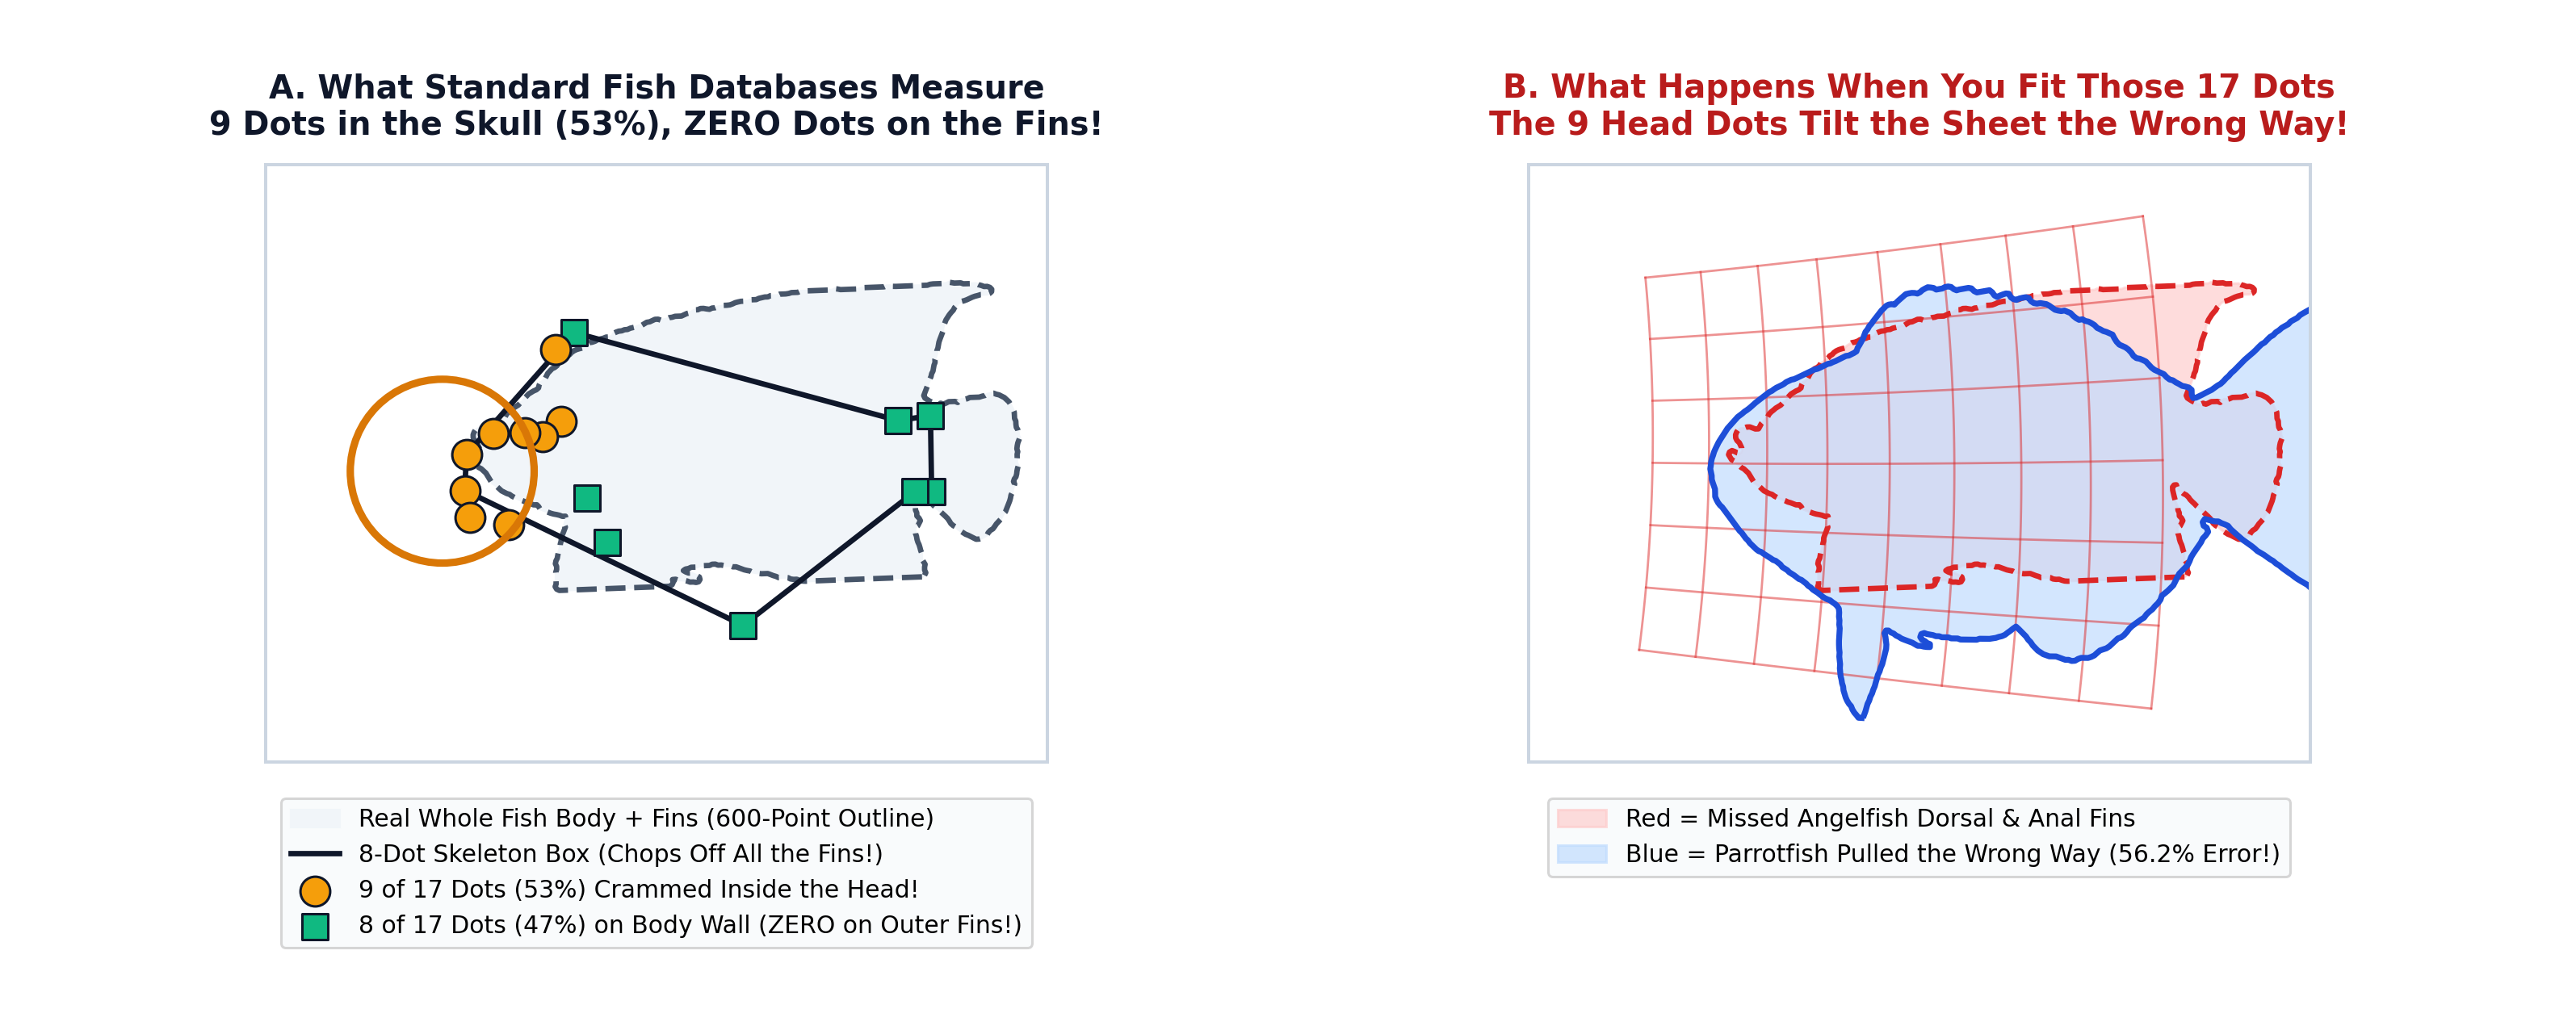
\includegraphics[width=0.99\textwidth]{guide_step2_17dot_head_trap.png}
  \caption{\textbf{Step 2 --- The ``17-Dot Head Seesaw Trap.''} \textbf{(A)} Standard fish databases put $9/17$ dots ($53\%$) inside the skull and $0$ dots on the outer fins. \textbf{(B)} When you fit a rubber sheet to those 17 dots, the 9 head dots act like a heavy seesaw and tilt the back of the sheet the wrong way ($56.2\%$ mismatch --- worse than not stretching the fish at all!).}
\end{figure}

\calloutbox{crimson}{crimsonbg}{Why the 17 Dots Failed}{%
Imagine trying to tailor a full-body wetsuit by measuring \textbf{9 points on someone's face} and \textbf{0 points on their arms or legs}. Because heads and fins evolve differently across fish families, forcing the rubber sheet to fit the 9 head dots swings the back of the sheet in the wrong direction!
}

% ============================================================================
\section*{Step 3: Mistake \#2 --- Why ``Just Stretching a Box'' Fails True Anatomy, and Why Thompson's Curves Win}

When we switch from 17 skeleton dots to a \textbf{600-point outline of the whole fish}, we have to be careful of a second trap: \emph{How do we know Thompson's slanted and curved grids are really needed, instead of just stretching a plain rectangle taller or wider (``Plain Box Stretch'')?}

\begin{figure}[H]
  \centering
  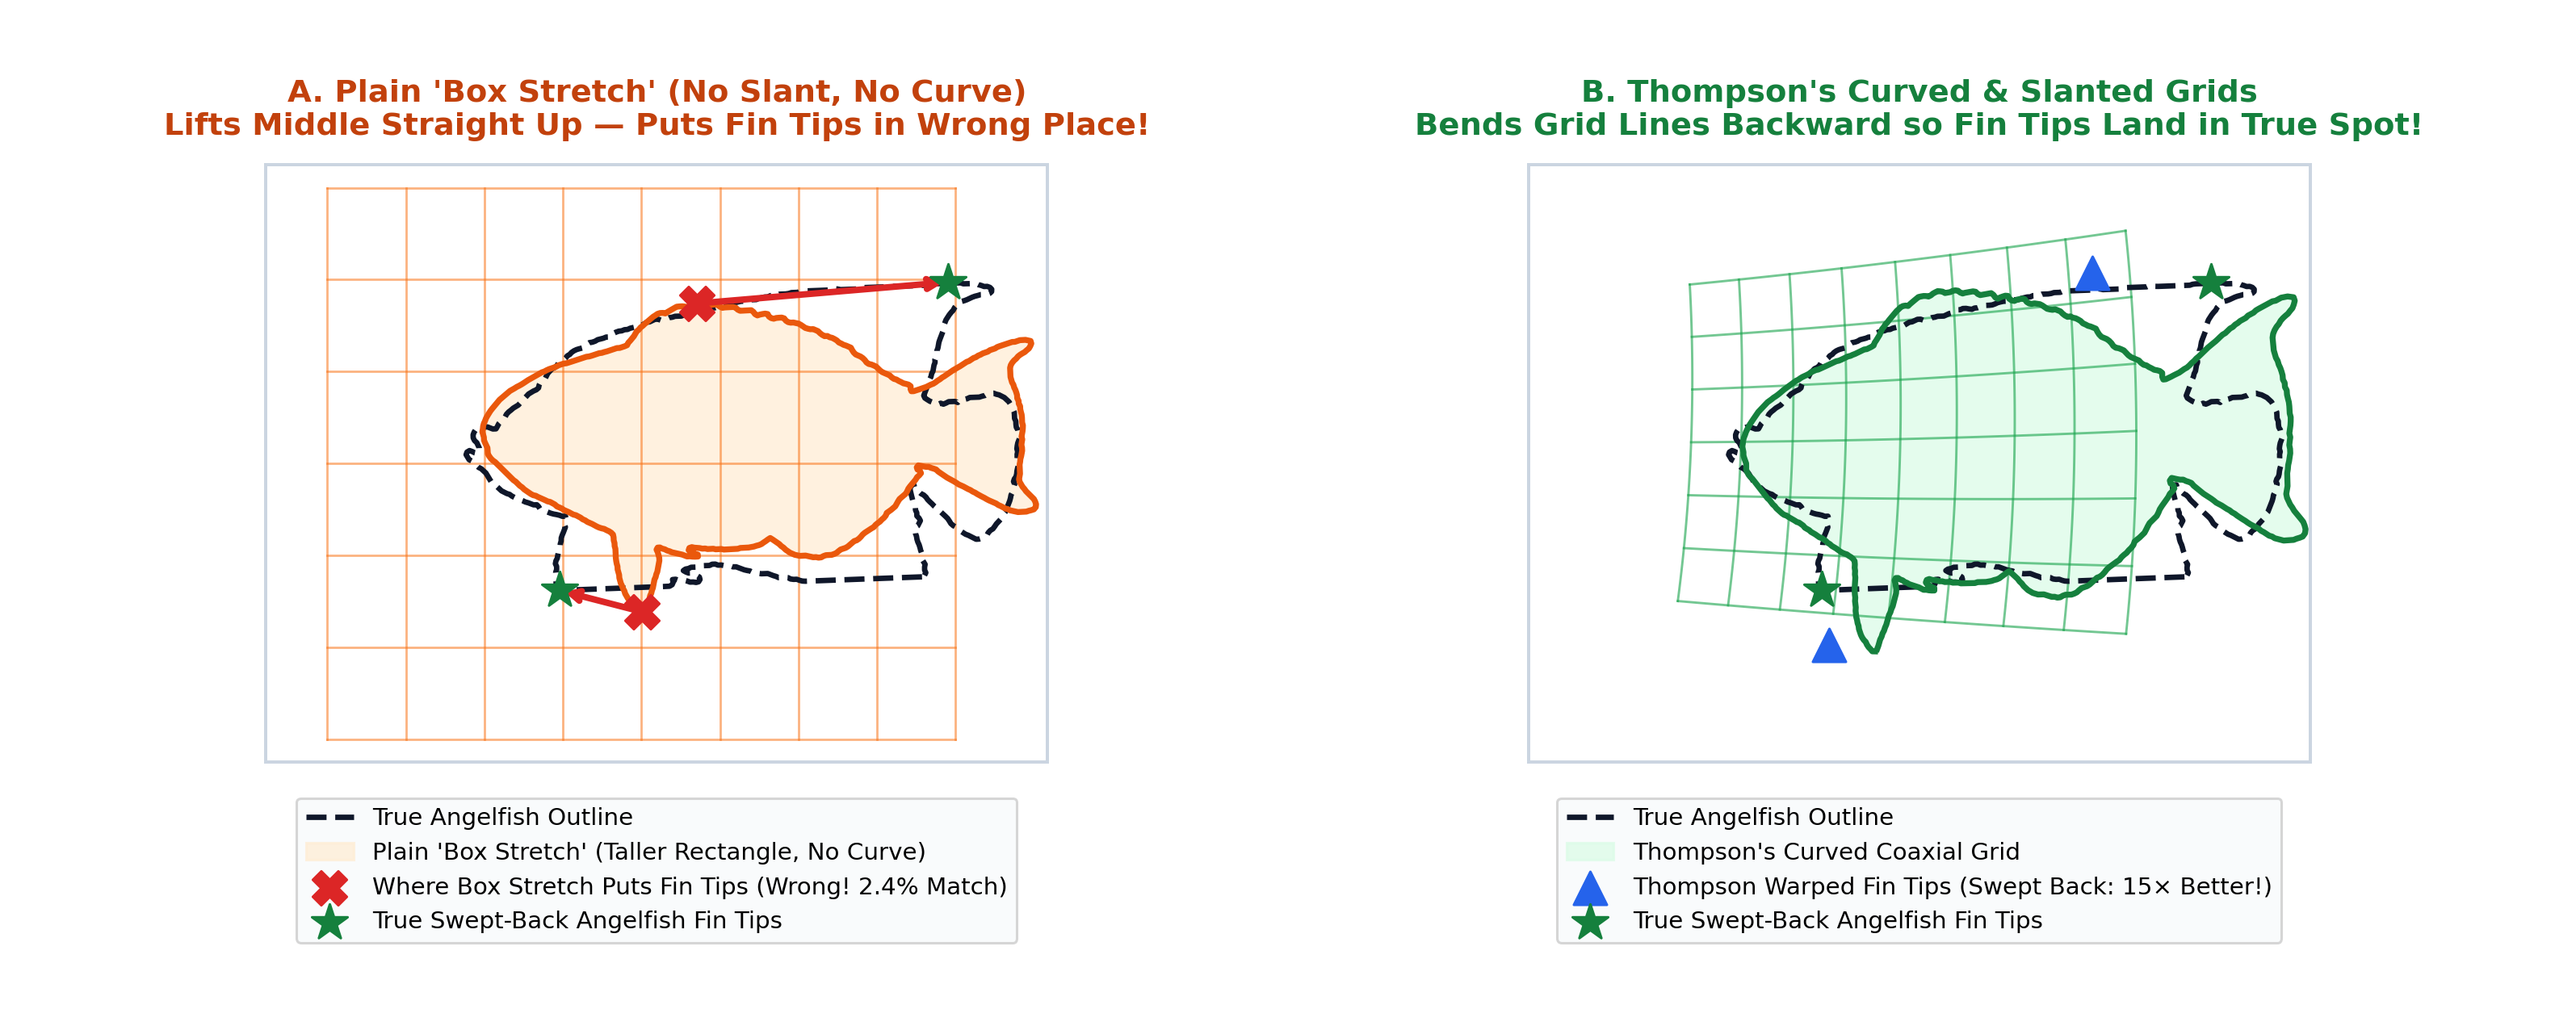
\includegraphics[width=0.99\textwidth]{guide_step3_box_cheat_vs_curves.png}
  \caption{\textbf{Step 3 --- Plain ``Box Stretch'' vs.\ Thompson's Curved Grids.} \textbf{(A)} A plain rectangular Box Stretch (no slant, no curve) lifts the middle of the back straight up (red \textbf{X}), missing the swept-back fin tips of the angelfish ($2.4\%$ accuracy). \textbf{(B)} Thompson's curved coaxial grid bends the grid lines backward so the fin tips land in their true swept-back position ($15\times$ more accurate!).}
\end{figure}

\begin{itemize}
  \item \textbf{The ``Shadow Cheat'':} If you only ask a computer to overlap two \textbf{unlabeled black shadows}, a plain rectangular Box Stretch can ``cheat'': on a pufferfish $\to$ ocean sunfish, it stretches the \emph{middle of the pufferfish's belly} straight up and down to cover the \emph{back fins} of the sunfish! And on a parrotfish $\to$ angelfish (Panel A above), a Box Stretch lifts the \emph{middle of the back} straight up (red \textbf{X}), missing the swept-back fin tips completely (\textbf{only $2.4\%$ match!}).
  \item \textbf{Why Thompson's Curved Grids Win:} Once you tell the computer which part of the outline is the \textbf{Dorsal Fin Tip}, which part is the \textbf{Anal Fin Tip}, and where the fins attach along the body (without the 9 internal skull dots), a plain Box Stretch fails, and \textbf{Thompson's slanted and curved grids jump by $+13\%$ to $+48\%$ accuracy} across all six 1917 pairs!
\end{itemize}

\newpage
% ============================================================================
\section*{Step 4: The Big Picture Across 10,303 Species --- Two Simple Rules of Fish Evolution}

To be sure our answer wasn't a fluke of just a few fish, we tested \textbf{three independent datasets} totaling \textbf{10,303 fish species across 987 genera and 440 families}. We found that fish evolution follows \textbf{two simple rules at the same time}:

\begin{figure}[H]
  \centering
  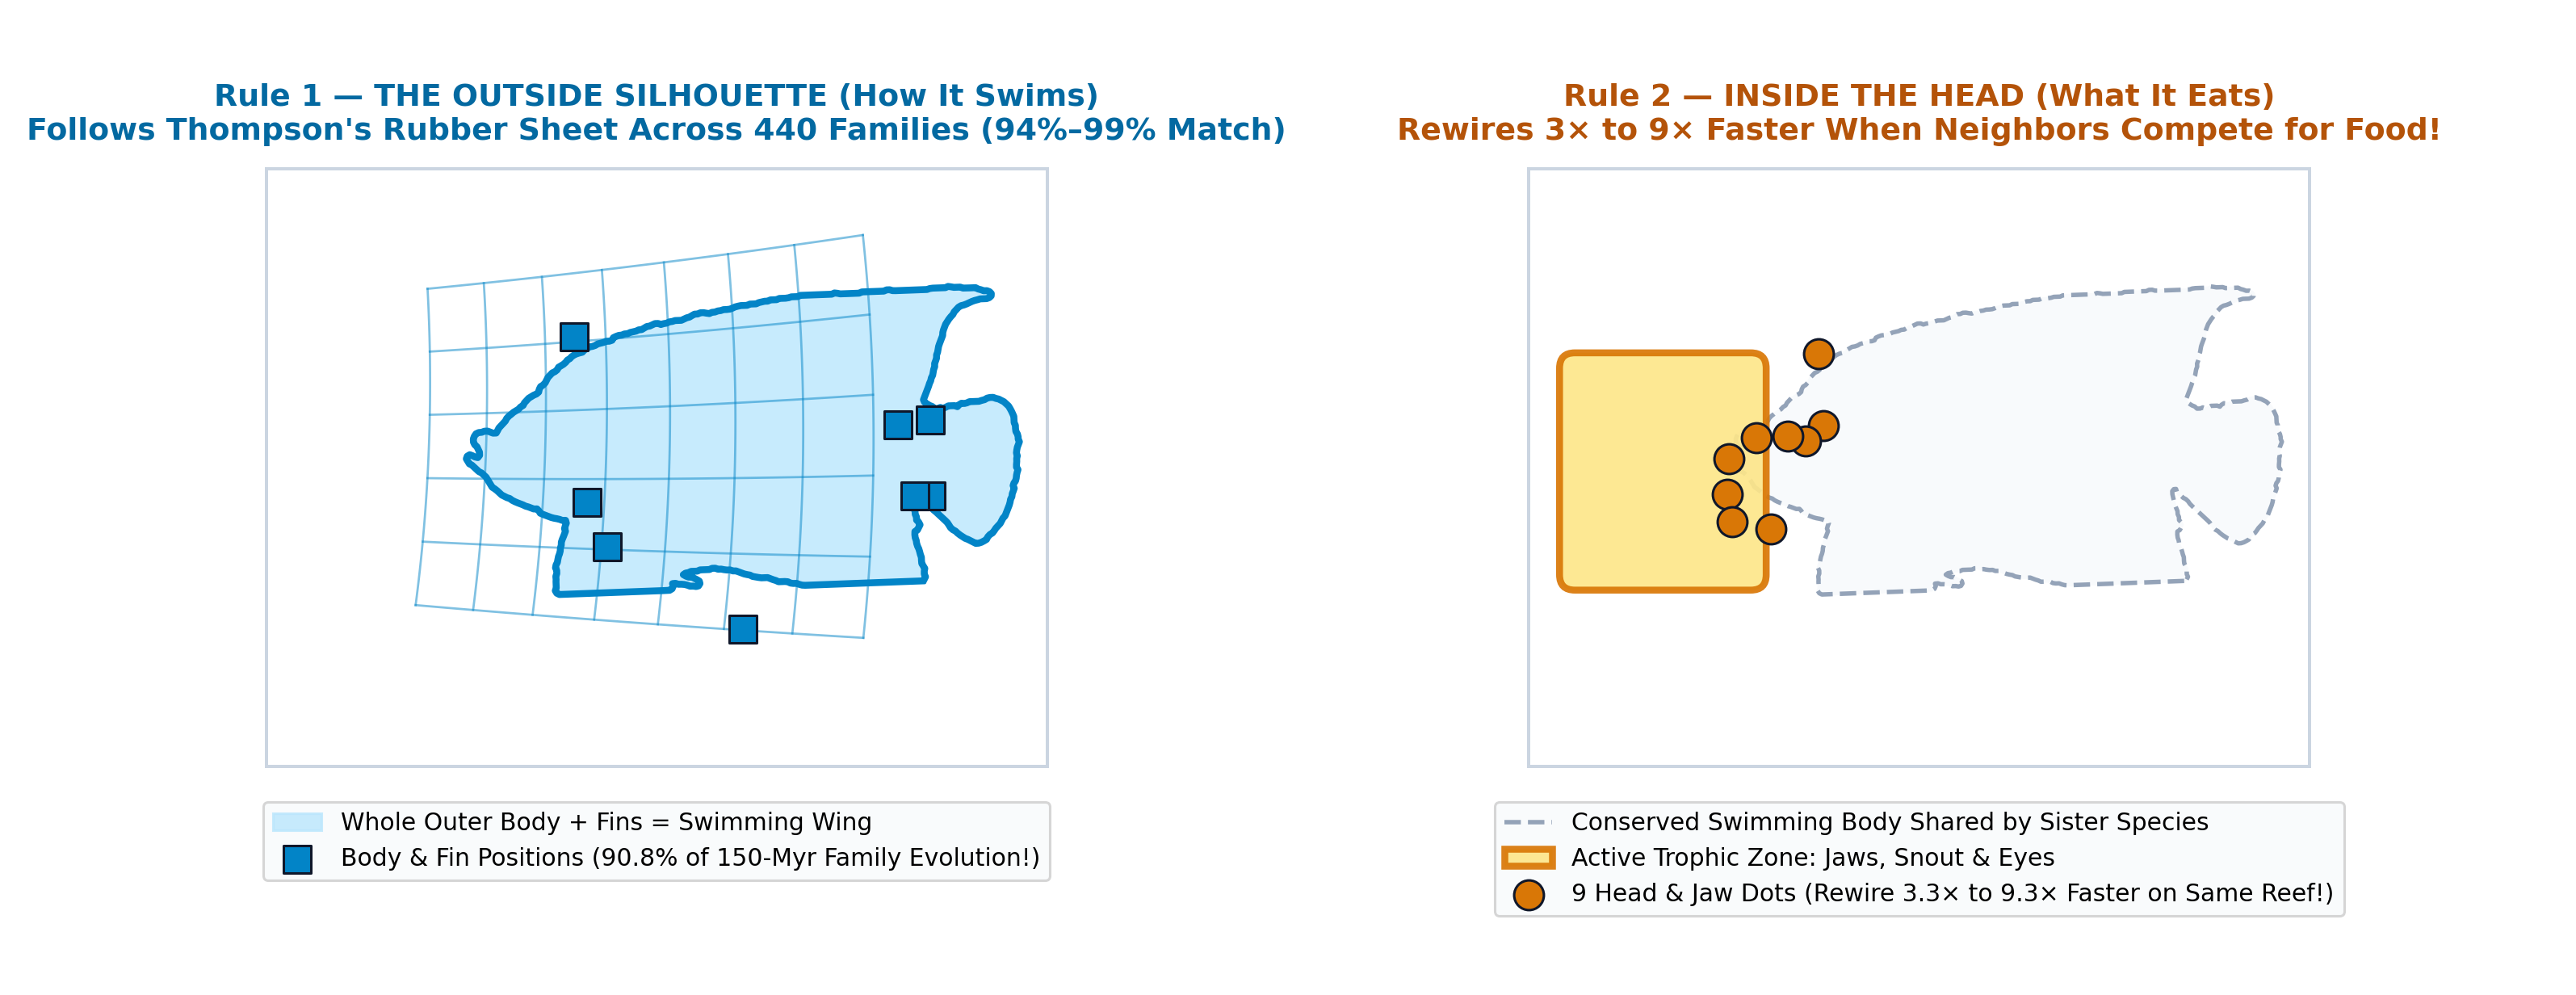
\includegraphics[width=0.99\textwidth]{guide_step4_outside_vs_inside_rules.png}
  \caption{\textbf{Step 4 --- The Two Rules of Fish Evolution Across 10,303 Species.} \textbf{Left (Rule 1 --- The Outside Silhouette):} The whole outer body and fins work together like a swimming wing and follow D'Arcy Thompson's curved rubber sheet across 440 families ($94\%\text{--}99\%$ alignment). \textbf{Right (Rule 2 --- Inside the Head):} When sister species live side-by-side on the same coral reef, their jaws, snouts, and eyes rewire $3.3\times$ to $9.3\times$ faster than their bodies so they can eat different foods without competing.}
\end{figure}

\calloutbox{sky}{skybg}{Rule 1 --- The Outside Silhouette (How the Fish Swims)}{%
Water doesn't flow around an invisible internal skeleton; it flows around the \textbf{whole outer silhouette} of the body and fins acting like an airplane wing. Over \textbf{150 million years across 440 fish families}, whole-body evolution follows D'Arcy Thompson's 8-knob rubber sheet ($93.5\%$ to $98.9\%$ alignment!). Even unrelated fish families separated by 100 million years take the \textbf{exact same Thompson highway} when they evolve to swim in the same kind of water.
}

\calloutbox{amber}{amberbg}{Rule 2 --- Inside the Head (What the Fish Eats)}{%
Why did the 9 head dots break the global rubber sheet? Because when closely related \textbf{sister species live side-by-side on the same coral reef}, they already have the same swimming body --- which means they would be fighting over the exact same food! To avoid competing, sister species rapidly rewire their \textbf{jaws, snouts, and eyes $3.3\times$ to $9.3\times$ faster than their bodies} ($85.4\%$ of within-genus evolution): one cousin evolves jaws to crunch coral, another sucks in tiny plankton, and another scrapes algae!
}

% ============================================================================
\section*{Step 5: The Final Scoreboard in Four Simple Numbers}

\begin{figure}[H]
  \centering
  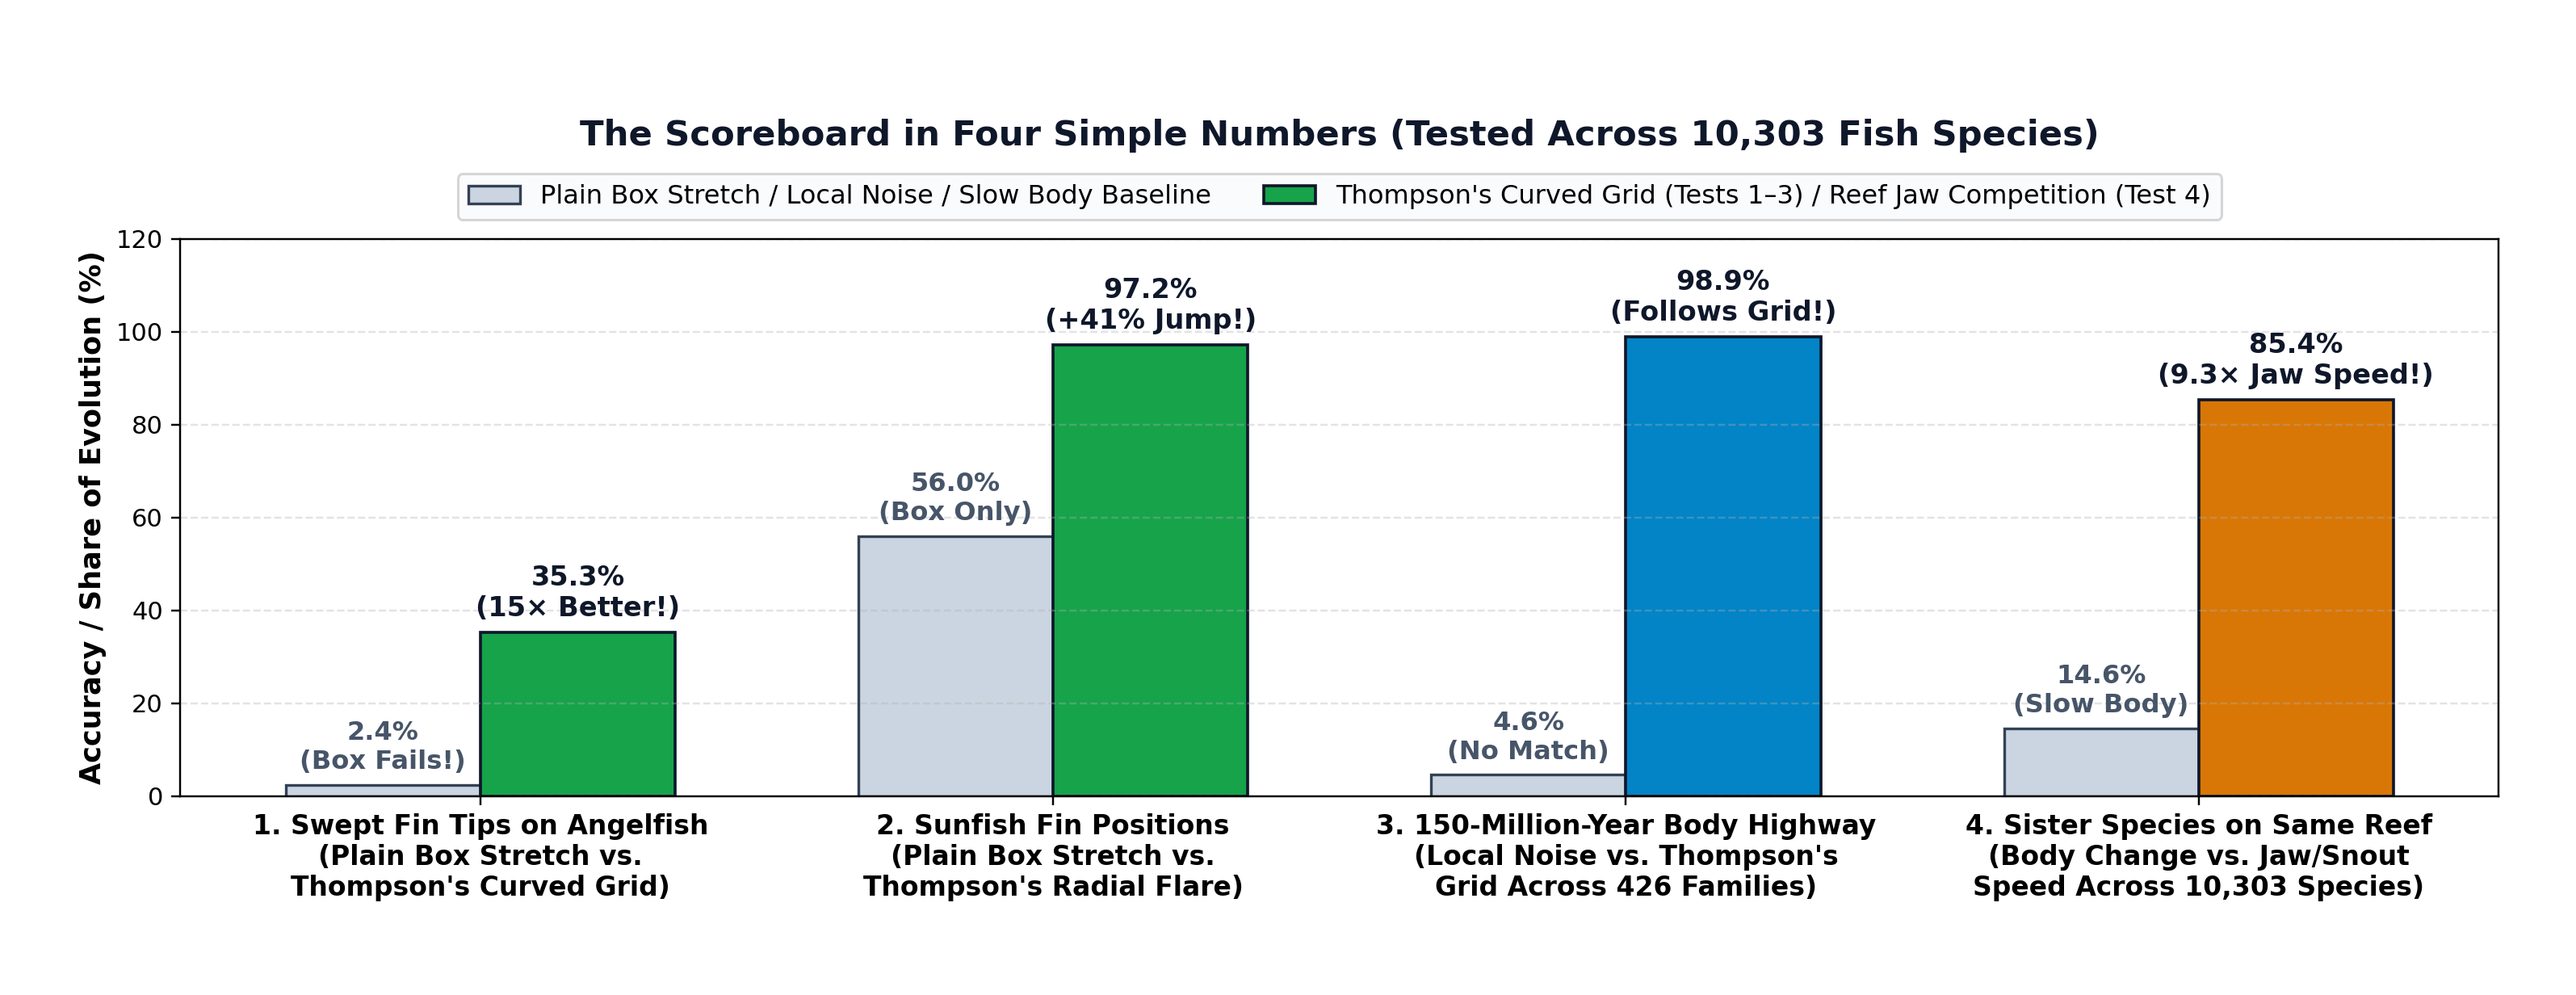
\includegraphics[width=0.99\textwidth]{guide_step5_10000_fishes_scoreboard.png}
  \caption{\textbf{Step 5 --- The Four-Number Scoreboard Across 6 Classic Pairs \& 10,303 Species.} Comparing plain Box Stretch / baseline assumptions (grey bars) against Thompson's curved grids (Tests 1--3) and reef jaw competition (Test 4).}
\end{figure}

\begin{table}[H]
\centering
\renewcommand{\arraystretch}{1.35}
\resizebox{\textwidth}{!}{%
\begin{tabular}{@{}p{0.28\textwidth}p{0.22\textwidth}p{0.22\textwidth}p{0.24\textwidth}@{}}
\toprule
\textbf{What We Tested} & \textbf{Plain Box / Baseline} & \textbf{Our Discovery} & \textbf{What It Means in Plain English} \\
\midrule
\textbf{1.\ Angelfish Swept Fin Tips} & $2.4\%$ (Box Fails) & $\mathbf{35.3\%}$ (\textcolor{emerald}{$\mathbf{15\times}$ Better}) & You need Thompson's curved circles to sweep the fin tips backward. \\
\textbf{2.\ Ocean Sunfish Fin Bases} & $56.0\%$ (Box Only) & $\mathbf{97.2\%}$ (\textcolor{emerald}{$\mathbf{+41\%}$ Jump}) & You need Thompson's exponential flare to match the giant tail-fins. \\
\textbf{3.\ 150-Myr Body Highway} & $4.6\%$ (Local Noise) & $\mathbf{98.9\%}$ (\textcolor{sky}{Follows Grid!}) & Across 426 families, whole body plans evolve along Thompson's grid. \\
\textbf{4.\ Reef Sister-Species Jaws} & $14.6\%$ (Slow Body) & $\mathbf{85.4\%}$ (\textcolor{amber}{$\mathbf{9.3\times}$ Jaw Speed!}) & Across 10,303 species, neighbors on the same reef rapidly rewire their jaws to share food. \\
\bottomrule
\end{tabular}%
}
\end{table}

\end{document}
